\documentclass[11pt,letterpaper]{article}

\usepackage[letterpaper,top=0.5in,bottom=0.5in,left=0.55in,right=0.55in]{geometry}
\usepackage{graphicx}
\usepackage{xcolor}
\usepackage{listings}
\usepackage{booktabs}
\usepackage{hyperref}
\usepackage{caption}
\usepackage{float}
\usepackage{titlesec}
\usepackage{amsmath}

\hypersetup{
    colorlinks=true,
    linkcolor=blue!60!black,
    urlcolor=blue!60!black,
}

\setlength{\parskip}{2pt}
\setlength{\parindent}{0pt}
\titlespacing*{\section}{0pt}{6pt}{2pt}
\titlespacing*{\subsection}{0pt}{4pt}{2pt}
\captionsetup{skip=2pt,font=small}

\graphicspath{{figures/}}

% -----------------------------------------------------------------------------
% Code listing styles
% -----------------------------------------------------------------------------
\definecolor{codebg}{RGB}{248,248,248}
\definecolor{codekw}{RGB}{0,0,180}
\definecolor{codecmt}{RGB}{0,120,0}
\definecolor{codestr}{RGB}{170,55,20}
\definecolor{codenum}{RGB}{120,120,120}

\lstset{
    language=C,
    basicstyle=\ttfamily\footnotesize,
    keywordstyle=\color{codekw}\bfseries,
    commentstyle=\color{codecmt}\itshape,
    stringstyle=\color{codestr},
    numbers=left,
    numberstyle=\tiny\color{codenum},
    stepnumber=1,
    numbersep=5pt,
    backgroundcolor=\color{codebg},
    frame=single,
    rulecolor=\color{black!30},
    tabsize=4,
    showstringspaces=false,
    breaklines=true,
    breakatwhitespace=false,
    breakindent=0pt,
    postbreak=\mbox{\textcolor{red}{$\hookrightarrow$}\space},
    captionpos=b,
    aboveskip=4pt,
    belowskip=4pt,
    xleftmargin=6pt,
    xrightmargin=2pt,
    columns=fullflexible,
    keepspaces=true,
    morekeywords={u32,s32,Xil_Out32,Xil_In32}
}

\lstdefinelanguage{VHDLsmall}{
    sensitive=false,
    morekeywords={architecture,begin,component,downto,end,entity,is,library,
        others,port,map,signal,std_logic,std_logic_vector,to,use,work,all},
    morecomment=[l]--
}

\lstdefinestyle{vhdlstyle}{
    language=VHDLsmall,
    basicstyle=\ttfamily\footnotesize,
    keywordstyle=\color{codekw}\bfseries,
    commentstyle=\color{codecmt}\itshape,
    numbers=left,
    numberstyle=\tiny\color{codenum},
    numbersep=5pt,
    backgroundcolor=\color{codebg},
    frame=single,
    rulecolor=\color{black!30},
    tabsize=4,
    breaklines=true,
    captionpos=b,
    aboveskip=4pt,
    belowskip=4pt,
    xleftmargin=6pt,
    xrightmargin=2pt,
    columns=fullflexible,
    keepspaces=true
}

\title{\vspace{-0.6in}\textbf{ECEC 661 -- Homework 4}\\
       \large CORDIC Square Root IP (AXI-Stream core + custom AXI-Lite IP) on Cora Z7-07S}
\author{Gary Pham \texttt{(gp492)}}
\date{\today}

\begin{document}
\maketitle
\vspace{-0.25in}

% =============================================================================
\section{Problem Statement}
% =============================================================================

Implement a Zynq PS+PL system that computes \(\sqrt{x}\) using the Xilinx
\textbf{CORDIC} IP configured for the \textbf{Square Root} function. Input
\(x\) is presented as an unsigned \textbf{2Q7} fraction on the lower ten bits
of a 16-bit word; output \(z=\sqrt{x}\) is an unsigned \textbf{1Q8} fraction on
the lower ten bits. Deliverables include HDL simulation of \texttt{user\_logic},
a packaged custom IP that maps software-visible \texttt{slv\_reg*} registers to
the core, a Vivado block design, and a bare-metal C test application with UART
evidence.

% =============================================================================
\section{CORDIC IP Configuration}
% =============================================================================

The Vivado IP Catalog instance \texttt{cordic\_0} (\texttt{xilinx.com:ip:cordic:6.0})
was configured to match the assignment (Square Root, parallel architecture,
maximum pipelining, unsigned fractional data, 10-bit in/out, truncate rounding):

\begin{table}[H]
    \centering
    \caption{CORDIC IP settings used for \texttt{cordic\_0}.}
    \label{tab:cordic_cfg}
    \small
    \begin{tabular}{ll}
        \toprule
        \textbf{Parameter} & \textbf{Value} \\
        \midrule
        Functional Selection & Square Root \\
        Architectural Configuration & Parallel \\
        Pipelining Mode & Maximum \\
        Data Format & UnsignedFraction \\
        Phase Format & Radians \\
        Input Width / Output Width & 10 / 10 \\
        Round Mode & Truncate \\
        \bottomrule
    \end{tabular}
\end{table}

The PG105 product guide describes how square-root mode interprets the Cartesian
slave stream as the radicand and produces \(\sqrt{x}\) on the master stream.

% =============================================================================
\section{Block Design}
% =============================================================================

Figure~\ref{fig:bd} shows the Vivado block diagram: Zynq~PS (UART0 on MIO~14/15),
\texttt{Processor System Reset}, an AXI interconnect or SmartConnect bridging
\texttt{M\_AXI\_GP0} to the custom slave \texttt{cordic\_sqrt\_axi\_0}, and
clock/reset distribution at \texttt{FCLK\_CLK0} (100\,MHz typical). The custom IP
was assigned base address \texttt{0x43C2\_0000} (64\,KB aperture), consistent with
\texttt{sw/main.c} and \texttt{xparameters.h}.

\begin{figure}[H]
    \centering
    
\includegraphics[width=\textwidth]{diagram.png}
    \caption{Vivado block design: Zynq PS, interconnect, and \texttt{cordic\_sqrt\_axi}
             AXI4-Lite peripheral.}
    \label{fig:bd}
\end{figure}

% =============================================================================
\section{User Logic and Custom IP}
% =============================================================================

\subsection{Assignment wrapper (\texttt{user\_logic.vhd})}

\texttt{user\_logic} preserves the required entity ports (\texttt{ck},
\texttt{aresetn}, \texttt{din\_tvalid}, \texttt{x[15:0]}, \texttt{dout\_tvalid},
\texttt{z[15:0]}) and instantiates \texttt{cordic\_0}. The Vivado CORDIC exposes
16-bit AXI-Stream \texttt{tdata} lanes even for a 10-bit configuration (byte
alignment); bits \([15{:}10]\) are zero-stuffed on input and ignored on output.
Bits \([9{:}0]\) carry the 2Q7 radicand and 1Q8 result respectively:

\begin{lstlisting}[style=vhdlstyle,caption={Core mapping in \texttt{Homework\_4/cordic\_sqrt/rtl/user\_logic.vhd} (excerpt).},label={lst:user_logic}]
s_tdata(9 downto 0)   <= x(9 downto 0);
s_tdata(15 downto 10) <= (others => '0');

U_CORDIC : cordic_0
    port map (
        aclk                    => ck,
        s_axis_cartesian_tvalid => din_tvalid,
        s_axis_cartesian_tdata  => s_tdata,
        m_axis_dout_tvalid      => dout_tvalid,
        m_axis_dout_tdata       => m_tdata
    );

z(9 downto 0)   <= m_tdata(9 downto 0);
z(15 downto 10) <= (others => '0');
\end{lstlisting}

\subsection{AXI4-Lite slave (\texttt{cordic\_sqrt\_axi\_v1\_0\_S00\_axi.vhd})}

The generated-style slave implements four 32-bit registers. Writes program \(x\)
and \texttt{din\_tvalid}; reads return \(z\) and \texttt{dout\_tvalid}. This
matches the assignment reference snippet (\texttt{mWriteReg}/\texttt{mReadReg}
offsets 0, 4, 8, 12):

\begin{table}[H]
    \centering
    \caption{Software register map (byte offsets from IP base).}
    \label{tab:regs}
    \small
    \begin{tabular}{clcp{7cm}}
        \toprule
        \textbf{Offset} & \textbf{Name} & \textbf{R/W} & \textbf{Purpose} \\
        \midrule
        \texttt{0x00} & \texttt{slv\_reg0} & R/W & \(x\): lower 10 bits = 2Q7 \\
        \texttt{0x04} & \texttt{slv\_reg1} & R/W & bit~0 = \texttt{din\_tvalid} \\
        \texttt{0x08} & \texttt{slv\_reg2} & R   & \(z\): lower 10 bits = 1Q8 \\
        \texttt{0x0C} & \texttt{slv\_reg3} & R   & bit~0 = \texttt{dout\_tvalid} \\
        \bottomrule
    \end{tabular}
\end{table}

Inside the slave, \texttt{core\_x <= slv\_reg0(15 downto 0)},
\texttt{din\_tvalid <= slv\_reg1(0)}, and the read multiplexer drives
\texttt{slv\_reg2}/\texttt{slv\_reg3} paths from \texttt{core\_z} and
\texttt{core\_dout\_tv}. Unlike Homework~3's accumulator, there is no
\texttt{slv\_reg\_wren}-as-clock trick: the CORDIC runs continuously on
\texttt{S\_AXI\_ACLK}.

% =============================================================================
\section{Behavioral Simulation}
% =============================================================================

\texttt{tb/tb\_user\_logic.vhd} exercises reset release, four consecutive samples
with \texttt{din\_tvalid} high (\texttt{0x080}, \texttt{0x040}, \texttt{0x008},
\texttt{0x000}), then compares pipelined outputs when \texttt{dout\_tvalid} is
asserted. Expected values match the specification (\texttt{0x100},
\texttt{0x0B5}, \texttt{0x040}, \texttt{0x000}).

\begin{figure}[H]
    \centering
    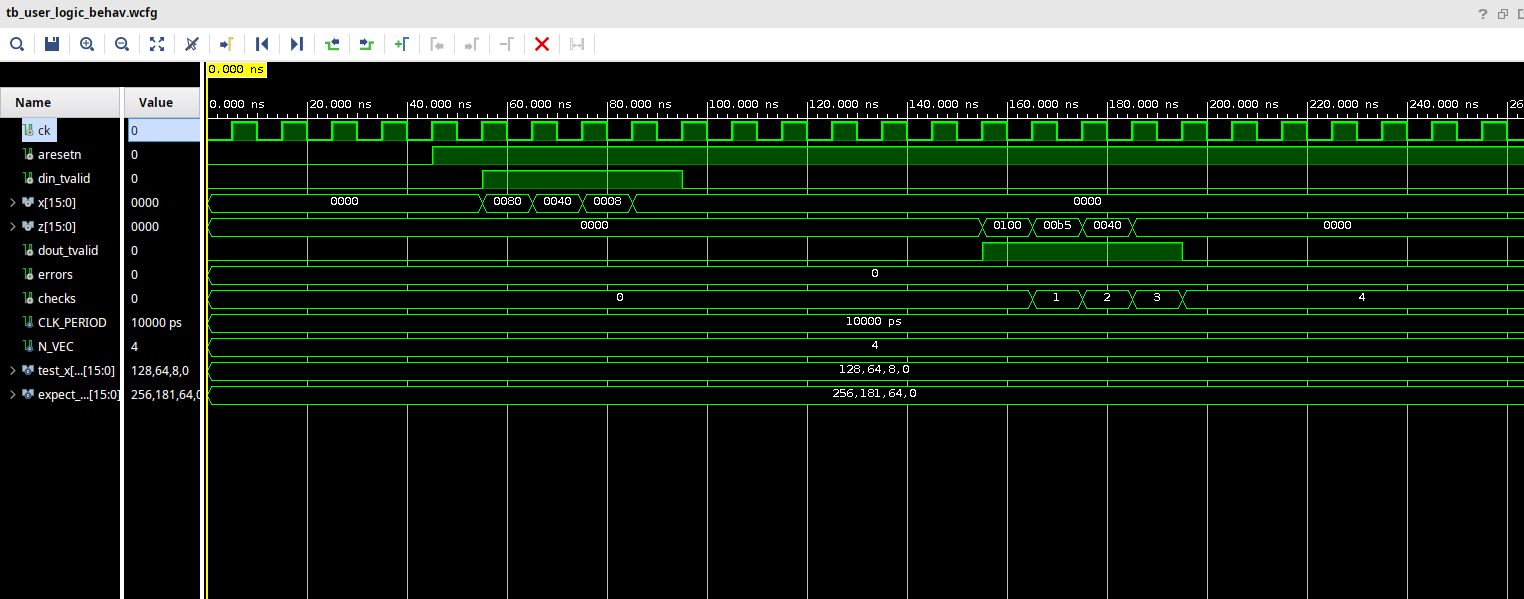
\includegraphics[width=\textwidth]{sim.png}
    \caption{Vivado xsim waveform: \texttt{ck}, \texttt{aresetn}, stream handshake,
             \texttt{x}, \texttt{dout\_tvalid}, and \texttt{z}.}
    \label{fig:sim}
\end{figure}

% =============================================================================
\section{Software (\texttt{main.c})}
% =============================================================================

The bare-metal application (\texttt{Homework\_4/cordic\_sqrt/sw/main.c}) follows
the assignment handshake exactly: write \(x\), assert \texttt{din\_tvalid}, spin on
\texttt{dout\_tvalid}, deassert \texttt{din\_tvalid}, then read \(z\). Fixed-point
decimals for the UART table are formatted without floating-point (\texttt{snprintf}
with scaled milli-fracts), and column widths align header, rule line, and rows.

\begin{lstlisting}[caption={Register handshake loop (core of \texttt{main.c}).},label={lst:handshake}]
for (int i = 0; i < N_TESTS; i++)
{
    CORDIC_SQRT_mWriteReg(BASEADDR, 0, test_vector[i]);  /* slv_reg0 = x */
    CORDIC_SQRT_mWriteReg(BASEADDR, 4, 1);               /* din_tvalid    */

    while (!CORDIC_SQRT_mReadReg(BASEADDR, 12))          /* dout_tvalid   */
        ;

    CORDIC_SQRT_mWriteReg(BASEADDR, 4, 0);               /* lower din_tv  */

    u32 x_in = CORDIC_SQRT_mReadReg(BASEADDR, 0);
    u32 z_out = CORDIC_SQRT_mReadReg(BASEADDR, 8);

    print_table_row(i, x_in, z_out, chk);
    ...
}
\end{lstlisting}

\textbf{Q-format display.} With \(x_{10}\) and \(z_{10}\) the 10-bit lanes,
\(\text{value}_x = x_{10}/128\) (2Q7) and \(\text{value}_z = z_{10}/256\) (1Q8).
The printed table labels columns \texttt{x dec 2Q7} and \texttt{z dec 1Q8}
accordingly.

\textbf{Test vectors.} Required cases \(1\), \(1/2\), \(1/16\) appear together with
extra checks (\(0\), \(1/4\), \(0.125\), \(3\)) to stress truncation and dynamic range.

% =============================================================================
\section{Hardware Results}
% =============================================================================

Figure~\ref{fig:vitis} shows UART output from the Vitis run on the Cora board:
seven rows, each \texttt{OK}, and a passing summary. This satisfies the PuTTY /
serial-monitor deliverable.

\begin{figure}[H]
    \centering
    
\includegraphics[width=0.92\textwidth]{vitis.png}
    \caption{UART trace from the bare-metal CORDIC square-root test (formatted table + summary).}
    \label{fig:vitis}
\end{figure}

Representative expected hex pairs for the three graded vectors:

\begin{table}[H]
    \centering
    \caption{Assignment reference vectors (2Q7 input \(\rightarrow\) 1Q8 \(\sqrt{x}\)).}
    \label{tab:vectors}
    \small
    \begin{tabular}{cccc}
        \toprule
        \(x\) (hex) & \(x\) decimal (2Q7) & \(z\) (hex) & \(z\) decimal (1Q8) \\
        \midrule
        \texttt{0x080} & 1.000 & \texttt{0x100} & 1.000 \\
        \texttt{0x040} & 0.500 & \texttt{0x0B5} & \(\approx 0.707\) \\
        \texttt{0x008} & 0.0625 & \texttt{0x040} & 0.250 \\
        \bottomrule
    \end{tabular}
\end{table}

% =============================================================================
\section{Conclusion}
% =============================================================================

The design wraps Xilinx \texttt{cordic\_0} in assignment-compliant \texttt{user\_logic},
packages it behind an AXI4-Lite slave with the reference register map, verifies the
three prescribed fractions (plus extra cases) in simulation and on silicon, and prints
a readable 2Q7/1Q8 table over UART for grading evidence.

\end{document}
